
\section{Teoria de Jogos, Coordenação e Planejamento}
\begin{frame}

\begin{center}
{\huge Capítulo 4 -- Teoria de Jogos e  Coordenação}

3 partes fundamentais:

\begin{enumerate}
  \item Teoria de Jogos
  \item Coordenação
  \item Planejamento
\end{enumerate}
Nesta ordem
\end{center}

\end{frame}

%-----------------------------------------------------------


%-----------------------------------------------------------


\section{Estratégias de Jogos}
\begin{frame}

    \frametitle{Teoria de Jogos}
    \begin{itemize}
    \pause
      \item SMA como um comunidade que coopera, disputa e \textit{compete} 
      \pause
      \item Asssim uma métrica entre todos os agentes (\textit{local}) é necessária para
      se levantar um valor \textit{global} de eficiência
    
    \end{itemize}
\end{frame}


%-----------------------------------------------------------



\subsection{Teoria de Jogos Aplicado a SMA}
\begin{frame}

    \frametitle{Dilema do Prisioneiro}
    \begin{block}
    Houve um assassinato e existem dois suspeitos, A e B. Se não se conseguir provar quem foi o assassino, a 
pena seria de apenas 6 meses por porte de arma.
Se um suspeito acusa o outro e este não se defender, então  será condenado a 10 anos.
Se o suspeito colaborar com a polícia sairá livre.
Se os dois se acusarem mutuamente a pena é de 5 anos para cada um.

\begin{itemize}
  
  \item Como os suspeitos não conhecem a \textit{Teoria dos Jogos}, o normal será que se acusem mutuamente
    
  \item Os suspeitos serão interrogados em separado e não tem acesso a(s) resposta(s) do outro

\item Sim, plural: rodadas ou jogadas de respostas!
\end{itemize}

    \end{block}
 
\end{frame}

%-----------------------------------------------------------

\begin{frame}

    \frametitle{Coletando os Dados : Dilema do Prisioneiro}
    
    
      \begin{center}
        \begin{tabular}{ccc} \hline \hline
             & Pris. B nega &  Pris. B delata   \\
        Prisioneiro A nega (silêncio)  &  Ambos condenados a 6 meses  & A é condenado a 10 anos e B é livre   \\ \hline \hline
         Prisioneiro A delata/acusa     & B é condenado a 10 anos e A é livre & Ambos são condenados a 5 anos \\ \hline 
         \hline \hline
        \end{tabular}
      \end{center}

\end{frame}


\begin{frame}

    \frametitle{Hipóteses: Dilema do Prisioneiro}
    
    
    \begin{itemize}
      \item  Vamos supor que ambos os prisioneiros são completamente egoístas e a sua única meta é reduzir a sua própria estadia na prisão. Como prisioneiros têm duas opções:
      
      \begin{enumerate}
         \item cooperar com o seu cúmplice e permanecer calado
         \item ou trair o seu cúmplice e confessar que foi o outro
       \end{enumerate}   
       
       \begin{itemize}
         \item   O resultado de cada escolha depende da escolha do cúmplice.     
         \item Infelizmente, um não sabe o que o outro escolheu fazer. 
       \end{itemize}
      %Incluso se pudessem falar entre si, não poderiam estar seguros de confiar mutuamente.
      

    
    
    
    \end{itemize}

Analisando os fatos:
\begin{quotation}
Se se esperar que o cúmplice escolha cooperar com ele e permanecer em silêncio, a opção óptima para o primeiro seria confessar, o que significaria que seria libertado imediatamente, enquanto o cúmplice terá que cumprir uma pena de 10 anos. Se espera que seu cúmplice decida confessar, a melhor opção é confessar também, já que ao menos não receberá a pena completa de 10 anos, e apenas terá que esperar 5, tal como o cúmplice. Se ambos decidirem cooperar e permanecerem em silêncio, ambos serão libertados em apenas 6 meses.
\end{quotation}

\end{frame}


%-----------------------------------------------------------

\begin{frame}
    \frametitle{Análise: Dilema do Prisioneiro}

   \begin{itemize}
     \item Confessar é uma estratégia dominante para ambos os jogadores. Seja qual for a escolha do outro jogador, podem reduzir sempre sua sentença confessando. 
   
  \item Por infelicidade para os prisioneiros, isto conduz a um resultado ruim, no qual ambos acusam seus companheiros e ambos recebem longas condenações. \textcolor{red}{Aqui se encontra o ponto-chave do dilema.} 
  
  \item O resultado das acusações individuais produz um resultado que não é óptimo no sentido de Pareto; existe uma situação tal que a utilidade de um dos detidos poderia melhorar (ou mesmo a de ambos) sem que isto implique uma piora para o resto. 
  
  \item Ou seja, o resultado no qual ambos os detidos não confessam (silêncio) dominam o resultado no qual os dois escolhem confessar.

   \end{itemize}
   
\end{frame}




\begin{frame}
    \frametitle{Análise: Dilema do Prisioneiro}

 \begin{itemize}
  
 
   \item Perspectiva de interesse ótima para o grupo (dos dois prisioneiros), o resultado correto é que  ambos cooperassem (entre si, ficando calados).
   Pois,  isto reduziria o tempo total de pena do grupo a um total de um ano (6 meses para cada um).

   \item  Qualquer outra decisão seria pior para ambos se se considerar conjuntamente.

\item Se um jogador tiver uma oportunidade para castigar o outro jogador ao confessar (delatar o outro), então um resultado cooperativo pode manter-se.
   \pause
   
   
\item Este jogo possui como solução do ponto de vista \textit{Ótimo de Pareto} a estratégia:
A e B negam (ficam calados!)

\pause
   
   
\item Este jogo possui como 
\textit{Equilíbrios de Nash} a estratégia: 
A e B delatam: neste caso, é o \textit{equilíbrio dominante}.

\item Porquê é chamado de \textit{Equilíbrios de Nash}?
     
 \end{itemize}
 
 %%Apesar disso, se continuarem no seu próprio interesse egoísta, cada um dos dos prisioneiros receberá uma dura pena.
 
% A forma iterada de este jogo (mencionada mais abaixo) oferece uma oportunidade para este tipo de castigo. Nesse jogo, se o cúmplice trai e confessa uma vez, pode-se castigá-lo traindo-o na próxima. Assim, o jogo iterado oferece uma opção de castigo que está ausente no modo clássico do jogo.


\end{frame}




%-----------------------------------------------------------
%-----------------------------------------------------------
%%% longe
\section{Coordenação}


\begin{frame}
\frametitle{Coordenação}



\end{frame}


%-----------------------------------------------------------


\subsection{Jogos de Coordenação}

\begin{frame}
\frametitle{Jogos de Coordenação}

pag 23


\end{frame}


%-----------------------------------------------------------
\subsection{Convenção Social}

\begin{frame}
\frametitle{Convenção Social}

pag 24


\end{frame}
%-----------------------------------------------------------

\subsection{Papel Social}

\begin{frame}
\frametitle{Papel Social}

pag 25


\end{frame}



%-----------------------------------------------------------
\subsection{Grafos de Coordenação}

\begin{frame}
\frametitle{Grafos de Coordenação}

pag 26


\end{frame}
%-----------------------------------------------------------


\subsubsection{Coordenação por Eliminação de Variáveis}

\begin{frame}
\frametitle{Coordenação por Eliminação de Variáveis}

pag 28


\end{frame}
%-----------------------------------------------------------


\subsubsection{Coordenação por Troca de Mensagens}

\begin{frame}
\frametitle{Coordenação por Troca de Mensagens}

pag 28


\end{frame}
%-----------------------------------------------------------

\section{Planejamento}


\begin{frame}
\frametitle{Fundamentos de Planejamento}



\end{frame}
%-----------------------------------------------------------


\subsection{Abordagens ao Planejamento Multiagente -- SMAs}

\begin{frame}
\frametitle{Abordagens ao Planejamento de SMAs}

\begin{block}{}
 
\begin{itemize}
  \item Coordenação central: controla todos os subplanos
  \item Esquemas de controle distribuído\\
        Conhecimento parcial dos planos de outros agentes
  \item Planejamento Global Negociado

\begin{itemize}
  \item Compartilhamento de todos os planos
  \item Ajuste local para a realização de objetivos comuns

\end{itemize}

\item Modelagem Explícita da Equipe de Agentes
\begin{itemize}
  \item Compromissos conjuntos
   \item Crenças, desejos e intenções comuns

\end{itemize}
\end{itemize}
\end{block}

\end{frame}

%-----------------------------------------------------


\subsection{Exemplos de Coordenação SMAs}

\begin{frame}
\frametitle{Exemplo de Coordenação SMAs}

\begin{figure}[!ht]
\centering
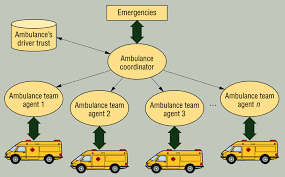
\includegraphics[height =.6\textheight,width=.7\textwidth]{figuras/coordenacao_agentes01.png}
\caption{Coordenação de agentes $\equiv $   SMA}
%\label{ag_01}
\end{figure}
 \end{frame}

%-----------------------------------------------------------

\begin{frame}
\frametitle{Exemplo de Coordenação SMAs}

\begin{figure}[!ht]
\centering
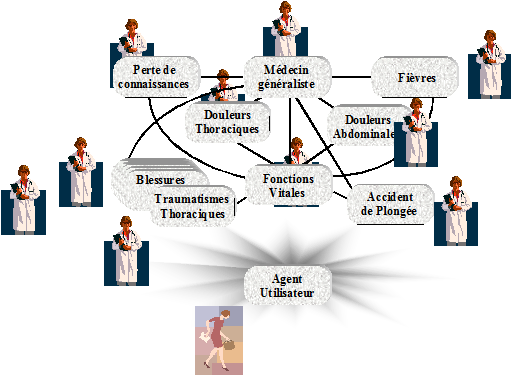
\includegraphics[height =.6\textheight,width=.7\textwidth]{figuras/coordenacao_agentes02.png}
\caption{Coordenação de agentes $\equiv $   SMA}
%\label{ag_01}
\end{figure}
 
\end{frame}


%-----------------------------------------------------------
